\chapter{Environement et jeu}

\section{Représentation du monde}
\subsection{Géométrie du monde}

        La premiere chose à faire était de définir des constantes, stuctures et variables qui allait nous servir tout au long du projet tel que : \\
        Les directions :
        \\
        \begin{center}
        \begin{multicols}{2}
        
            NORTH \\ NEAST  \\ NWEST \\ WEST \\ SOUTH \\ SWEST \\ SWEST \\ EAST  
        
        \end{multicols}
        \end{center} 
        Le type de couleur de la case :
        \begin{center}
            NO-COLOR \hspace{1cm} WHITE \hspace{1cm} BLACK \\
        \end{center}
        L'occupant de la case :
        \begin{center}
            NO-SORT \hspace{2cm} SIMPLE-PAWN \\ 
        \end{center}
        Cette catégorie est voué à s'agrandir au vu de l'ajout de différentes sorte de pions par la suite. \\\\
        Egalement nous avons besoin des variables du monde :
        \begin{center}
            taille: WORLD-SIZE longueur: WIDTH largeur: HEIGHT Nombre de cases Max: UNIT-MAN nombre de joueurs: NB-PLAYERS
        \end{center}
        Avec ces variables on a créé la structure "world" qui nous permet d'assigner à chaque case du monde sa couleur et son occupation ce qui nous servira grandement dans la suite du jeu.\\
\subsection{Plateau de jeu}
        Il faut definir un plateau de jeu pour l'utilisateur. Nous avons decidé de faire celui-ci de forme torique afin rendre le jeu plus modulable. Il a donc fallut nous affranchire des effets de bord à l'aide de modulo. Ce choix a aussi été fait pour des raisons d'entisipation des futures modifications qui seront plus faciles en partant d'un modèle très généraliste tel que le tore.
        \begin{center}
        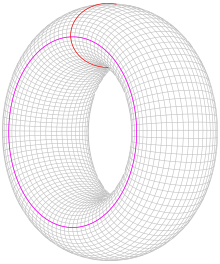
\includegraphics[scale=0.3]{tor.png}
        \end{center}
        
        
        Nous avons également pris par défault des relations entre les cases de type hexagonale(figure 1.a) comme il nous l'était imposé en début de projet. Cependant dans le cadre d'un achievement nous avons également implémenté un changement de térrain qui impact les relations faisant passer de case octogonale à des cases carré (figure 1.b)ou triagulaire (figure 1.c). Ces changements arrivent tout les x tours en focntion de la demande du joueurs.
\begin{figure}[htbp]
\centering
\begin{subfigure}{0.3\textwidth}
\centering
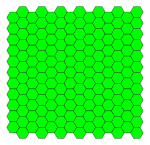
\includegraphics[width=\textwidth]{plateauhexa.png}
\caption{Pavage hexagonale}
\label{label_de_l_image_1}
\end{subfigure}
\quad
\begin{subfigure}{0.3\textwidth}
\centering
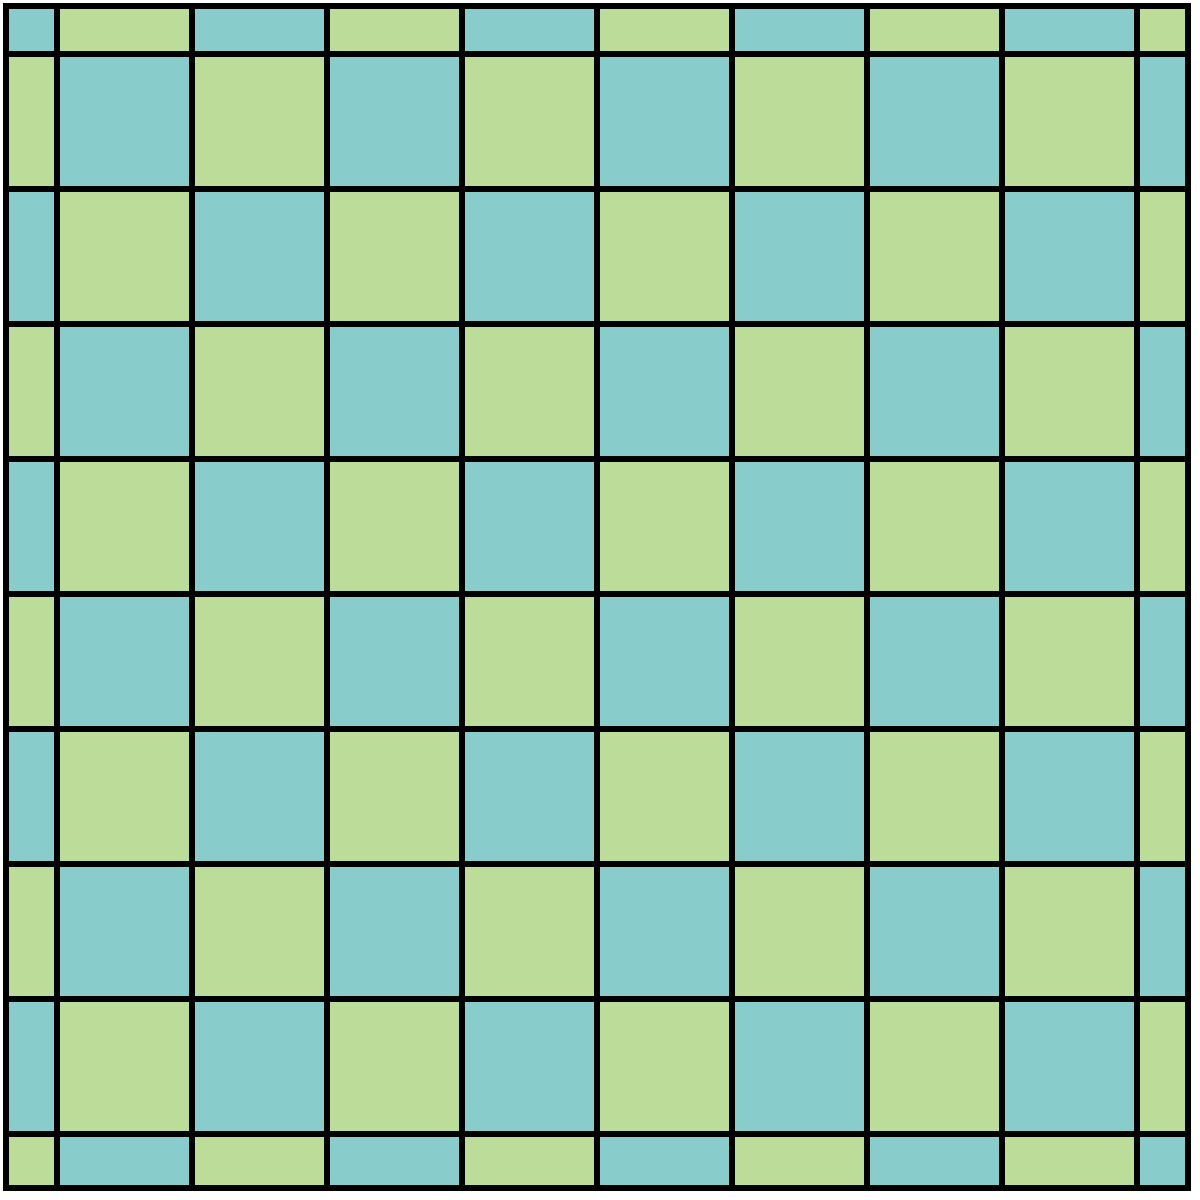
\includegraphics[width=\textwidth]{quadrillage.png}
\caption{Pavage carré}
\label{label_de_l_image_2}
\end{subfigure}
\quad 
\begin{subfigure}{0.3\textwidth}
\centering
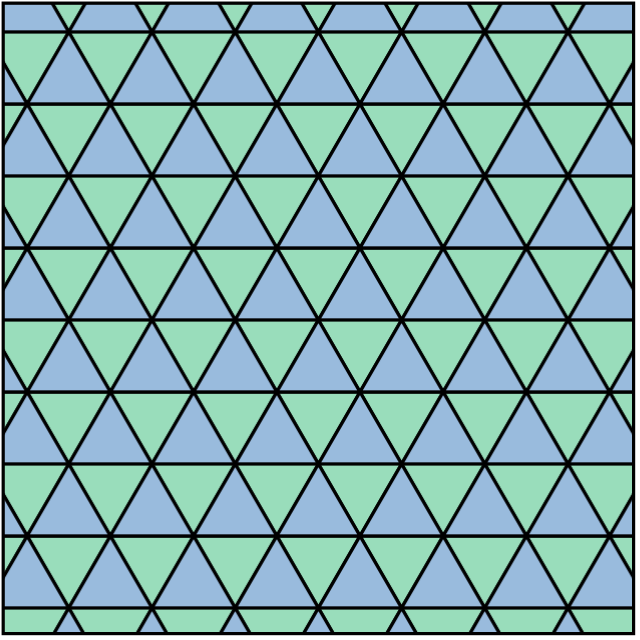
\includegraphics[width=\textwidth]{plateautri.png}
\caption{Pavage Triangulaire}
\label{label_de_l_image_3}
\end{subfigure}
\caption{Pavages disponible dans notre jeu}
\label{label_de_la_figure 1}
\end{figure}


\section{Pièces et joueurs}
\subsection{Pièces}
 Pour les pièces premièrement nous avons choisi de simple pions, pouvant se déplacer d'une seul case seulement si celle-ci est vide. Par la suite on a incorporé au jeu d'autres pieces le rendant plus interessant. Chaque piece a ses spécialités.\\ 
        C'est pour cela que nous avons créé une structure qui rend les pieces modulable. Chaque piece appartenant à cette structure est définit par : 
        \begin{itemize}
            \item Son joueur : 1 ou 2 
            \item Son nombre de déplacement : choisis en amont par le maitre de la partie
            \item Sa couleur : White ou Black 
            \item Son type : Pion, Tour, etc
            \item Sa position : [0 ; UNIT-MAX-1]\\
        \end{itemize}

        Le Pion : (insérer image) \\
        Le pion est la piece basique du jeu ayant un seul mouvement dans la direction de son choix. Cependant il est possible d'en faire une dame en augmentant son nombre de mouvement disponoble dans les parametres afin qu'il puisse se déplacer à la maniere d'une dame aux echècs.\\
        
        La Tour : ( insérer image )\\
        Elle peut comme aux échecs se déplacer seulement en direction des points cardinaux. Nous avons décidé de limiter ses déplacement au Max(longueur du plateau, largeur du plateau) car tant donné l'apparence torique de notre plateau de jeux ses movements pourrait être infinis.\\
        \\
        L'éléfun : (insérer image)\\
        Il se déplace uniquement suivant les 4 directions cardinales et possède dans le cas de base deux déplacements.
        \\
        Le Roi premier : (insérer image)\\
        Il se téléporte directement sur une case première si celle-ci n'est pas occupé par un autre pion.

\subsection{Joueurs}
\subsection{Formations de départ}
        Nous avons mis en place deux formations de départs différentes, une premiere classique qui resemble aux echecs en prennant en concidération la forme torique de notre plateau. \\
        La deuxième elle est plus anarchique et présente le plateau sous forme de champs de bataille avec deux énorme blocs de pièces séparé par des tranchés. \\
        Ces deux type de formation son modulable dans les pieces qui les composes car il est possible de choisir le nombre et le type de pieces "spécials" de la formation le reste est complété par des pions. 
        
\section{Boucle de jeu}
\subsection{Sélection des options}
\subsection{Déroulement d'une partie}
\subsection{Conditions de victoire}